\documentclass[12pt]{article}
\expandafter\def\csname
ver@l3backend.sty\endcsname{}

\usepackage{geometry}
\usepackage[hidelinks]{hyperref}
\usepackage{setspace}
\usepackage{amsmath}
\usepackage{amsthm}
\usepackage{amssymb}
\usepackage{mathtools}
\usepackage{xcolor}
\usepackage{graphicx}
\usepackage[utf8]{inputenc}
\usepackage{fontspec}
\usepackage{l3backend}
\usepackage{polyglossia}
\usepackage{testhyphens}
\usepackage{pgffor}

\setmainlanguage{finnish}
\addto\captionsfinnish{\renewcommand{\figurename}{Kuvio}}

\newcommand{\datalahde}[1]{\input{../plots/eurostat_statfin/#1_selite.txt}\unskip} 
\newcommand{\captionselite}[1] {\textit{\footnotesize{#1}}}

\newcommand{\komissiodatalahde} {Datalähde: \href{https://webgate.ec.europa.eu/empl/redisstat/databrowser/product/page/LMP_EXPME$FI}{\textcolor{blue}{https://webgate.ec.europa.eu/empl/redisstat/databrowser/product/page/LMP\_EXPME\$FI}}}

\newcommand{\seliteduration}[1] {\input{../plots/durations/#1_selite.txt}}

 \geometry{
 a4paper,
 % total={165mm,230mm},
 left=25mm,
 top=25mm,
 right=25mm
 }
 
\begin{document}



\noindent \textbf{Työvoimapalvelujen kustannukset} \par
\vspace{0.5cm}

\noindent Juho Alasalmi{\par}
\noindent \href{mailto: juho.alasalmi@ptt.fi}{\textcolor{blue}{juho.alasalmi@ptt.fi}}{\par}
\noindent Pellervon Taloustutkimus {\par}

\vspace{0.5cm}
\setstretch{1.2}

\section{Kokonaiskustannukset}

Tarkastelemme ensin kunkin työvoimapalvelun kokonaiskustannuksia (XTOT). Kustannukset ovat inflaatiokorjattu vuoden 2021 hintoihin käyttäen elinkustannusindeksiä.\footnote{\href{https://statfin.stat.fi/PxWeb/pxweb/fi/StatFin/StatFin__khi/statfin_khi_pxt_11xm.px/}{\textcolor{blue}{https://statfin.stat.fi/PxWeb/pxweb/fi/StatFin/StatFin\_\_khi/statfin\_khi\_pxt\_11xm.px/}}} Kuvio \ref{fig:sk230923t} esittää kokonaiskustannukset.

\begin{figure}
\centering
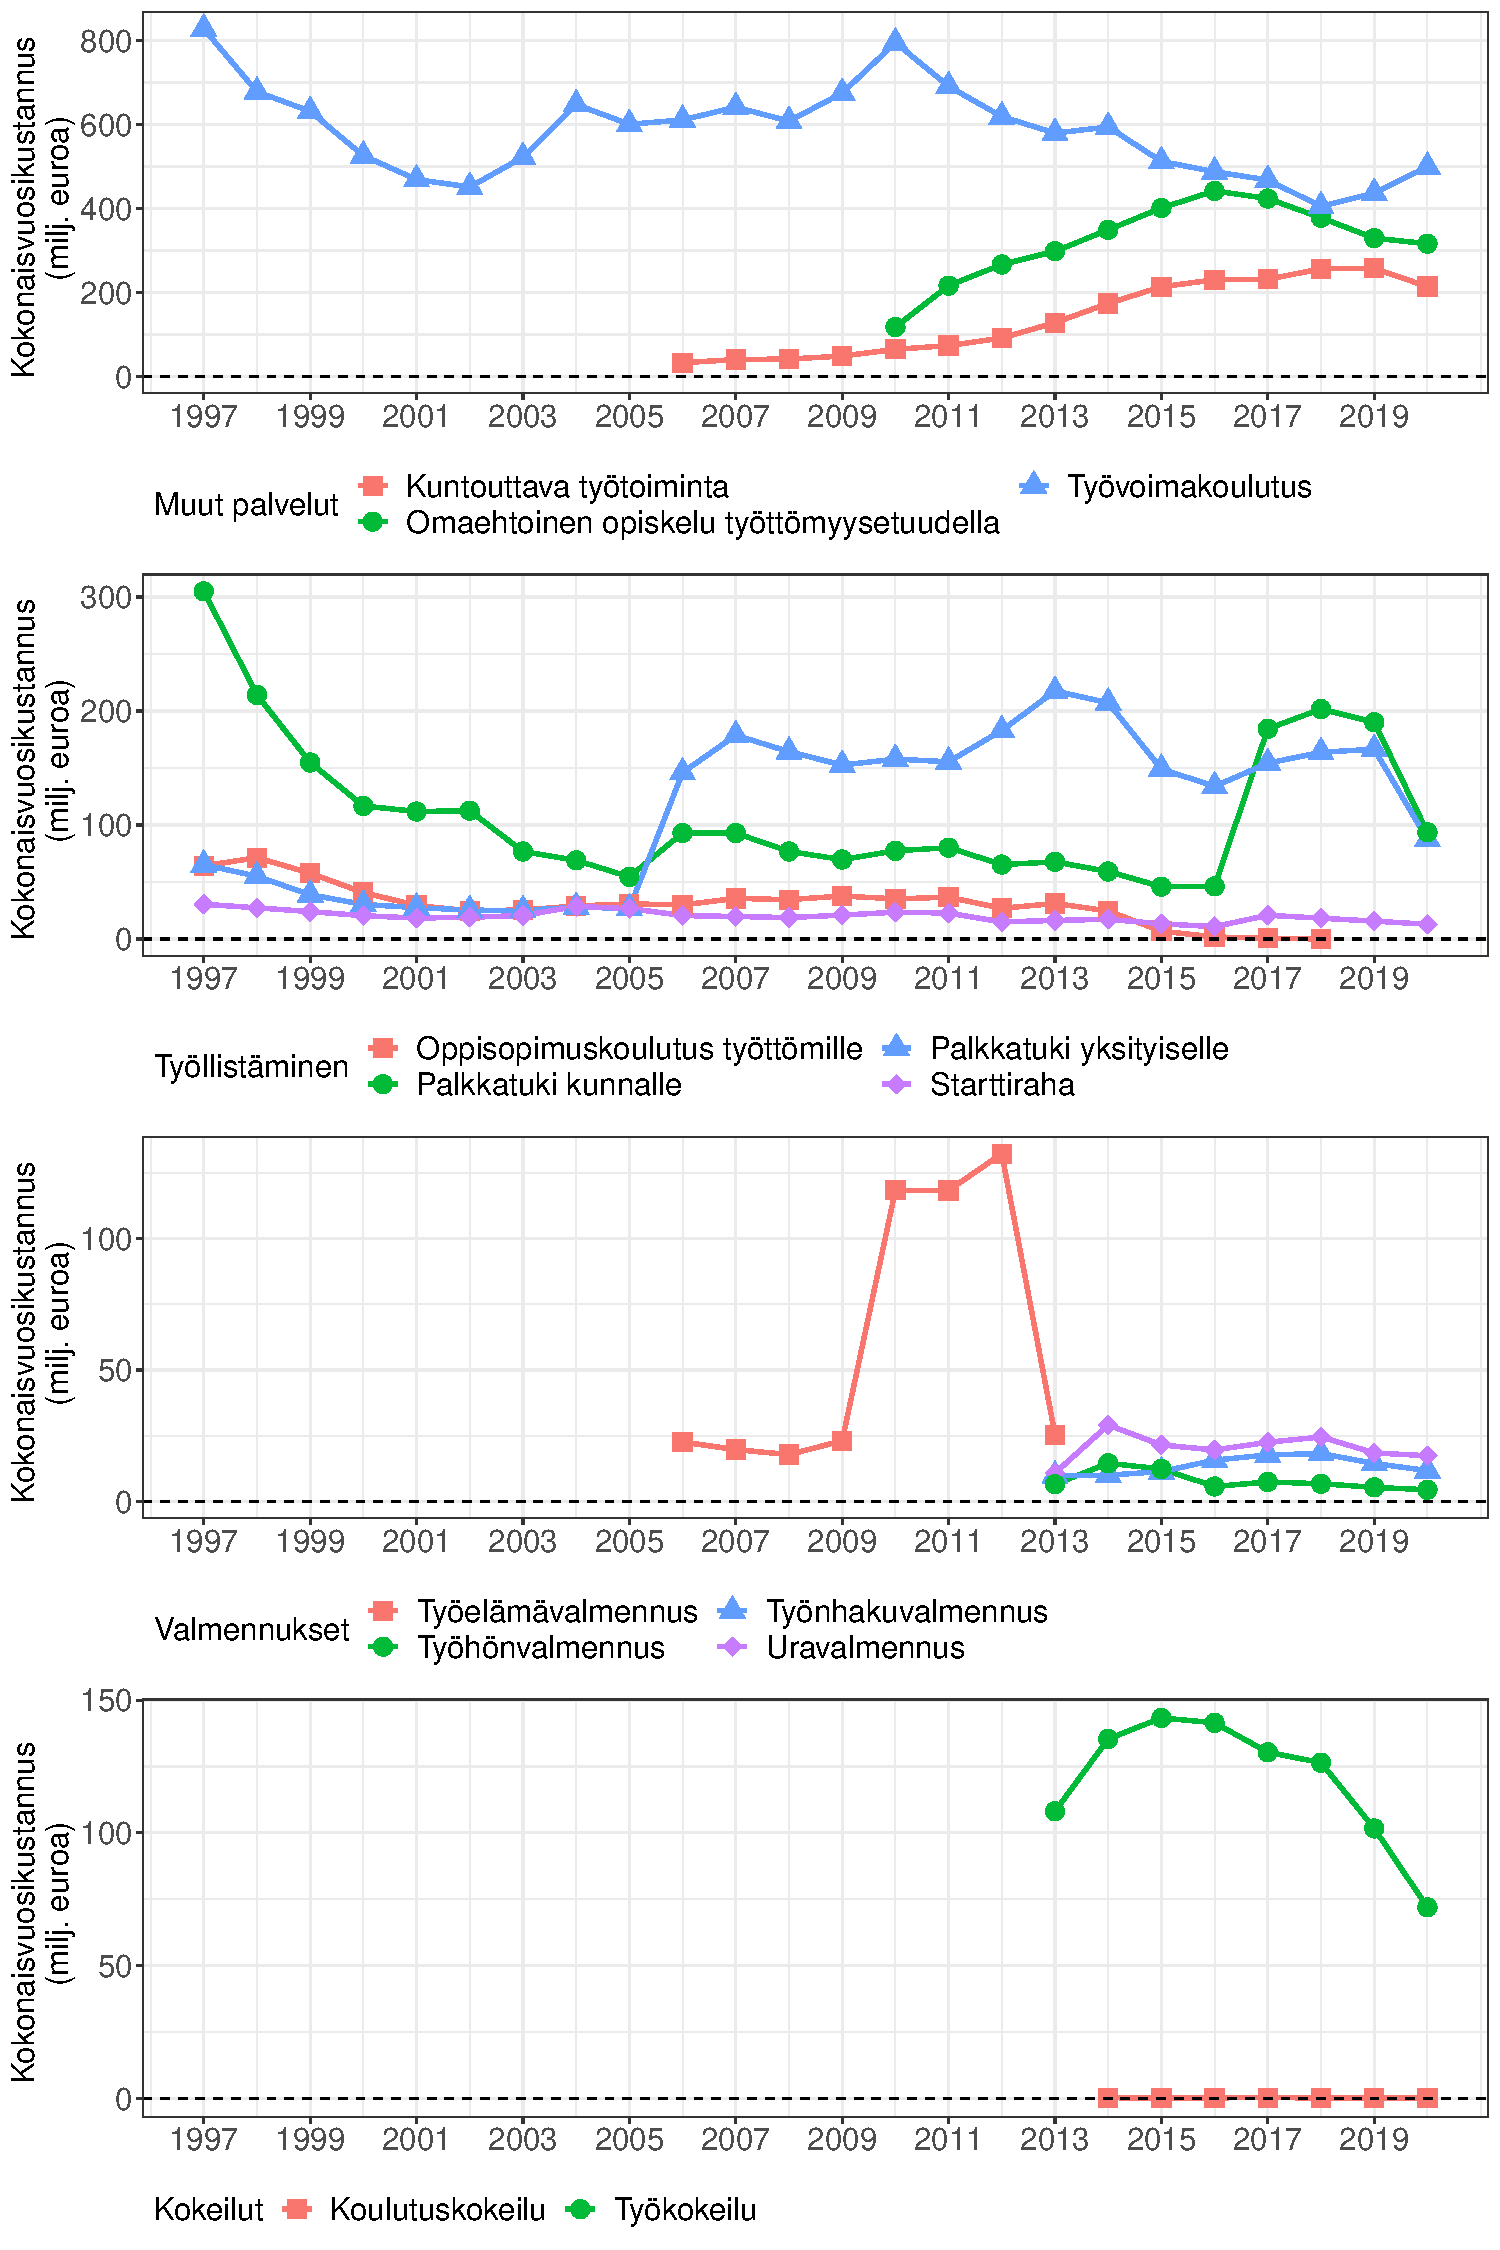
\includegraphics[scale = 0.6]{../plots/costs/total_costs.pdf}
\caption{Kokonaiskustannukset. \newline \captionselite{\komissiodatalahde}}
   \label{fig:sk230923t}
\end{figure}

\section{Aikakustannukset}

Palvelujen kokonaiskustannukset luonnollisesti riippuvat osallistujamääristä. Kustannukset myös riippuvat palvelujen kestoista. Pitkäkestoiset palvelut tuottavat enemmän kustannuksia kuin lyhytkestoiset. Ottamatta huomioon eri palvelujen erilaisia kestoja, eri palvelujen kustannusten vertaaminen ei välttämättä anna oikeaa kuvaa siitä kuinka kallista palvelujen tuottaminen on. Palvelujen erilaiset kestot voidaan ottaa huomioon vertailemalla kunkin palvelun tietyssä ajassa tuottamia kustannuksia. Yllä esitety kokonaiskustannukset kuvaavat, kuinka paljon kukin palvelu tuottaa kustannuksia vuodessa. Palvelussa olevien keskimääräinen määrä puolestaa kuvaa kuinka monta henkilöä palvelua keskimäärin kullakin hetkellä käyttää. Siten yhden henkilön osallistuminen vuoden ajan kustantaa XTOT / STK. Nämä vuosikohtaiset kustannukset ovat esitetty Kuviossa \ref{fig:dl2092g}.

\begin{figure}
\centering
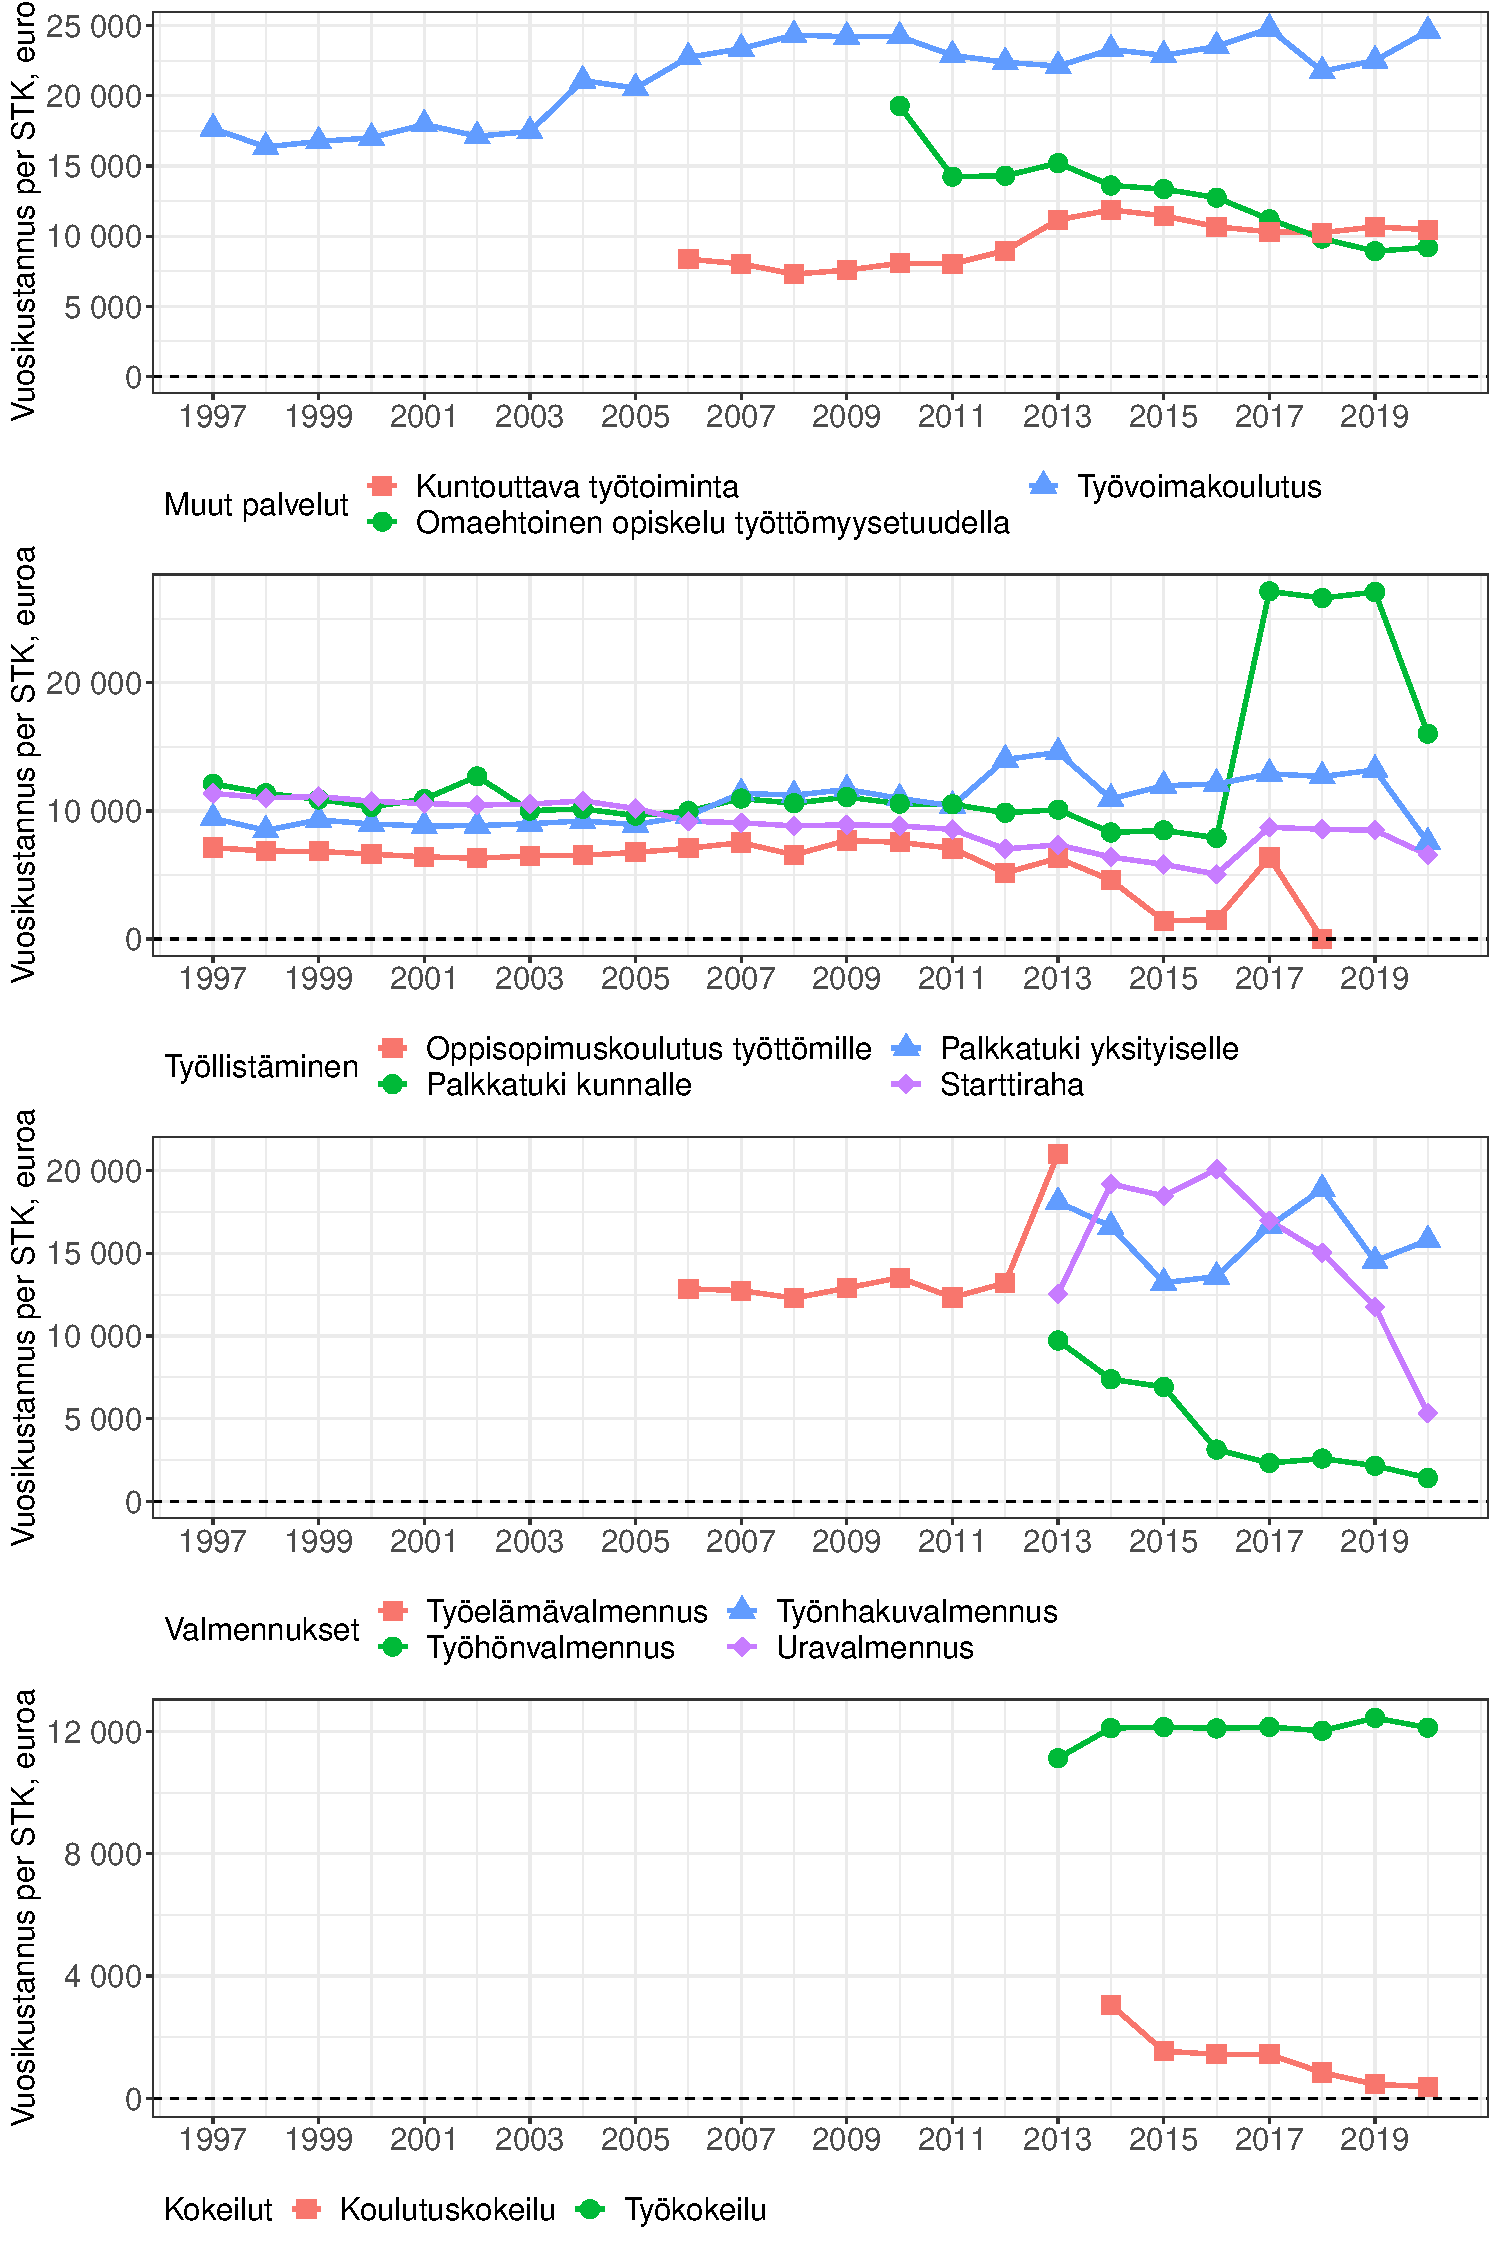
\includegraphics[scale = 0.6]{../plots/costs/annual_per_stock_costs.pdf}
\caption{Vuosikohtaiset kustannukset. \captionselite{Datalähde: kuten Kuvio \ref{fig:sk230923t}. Kirjoittajan omat laskelmat.}}
   \label{fig:dl2092g}
\end{figure}

\section{Osallistumiskustannukset}

Palveluun osallistumisen kustannus on siitä koituva kustannus ajassa kerrottuna palveluun osallistumisen kestolla. Jos palveluun $N$ henkilön palveluun osallistuminen tuottaa kustannuksia $x$ euroa kuukaudessa, ja palvelu keskimäärin kestää $T$ kuukautta, niin yhden henkilön osallistuminen tuottaa $x/N$ euroa kustannuksia kuukaudessa ja yhden henkilön osallistuminen palveluun tuottaa kustannuksia $x/N \times T$ euroa.

\subsection{Osallistumisen kesto}

Työvoimapalveluihin osallistumisen kestoja voidaan arvioida virta- ja varantosuureiden avulla. Jos palveluun osallistumisen kesto on $T$ päivää, silloin palvelussa olevien määrä (STK) ajanhetkellä $t$ on palvelussa ajanhetkillä $t - (T-1), ..., t$ aloittaneiden määrä (ENT). Siten 
\begin{align}
 \textup{STK} = T \times \textup{ENT} \iff T = \dfrac{\textup{STK}}{\textup{ENT}}
\end{align}
Toisaalta, STK ajanhetkellä $t$ on ajanhetkillä $t+1, ..., t + T$ palvelussa lopettaneiden määrä (EXIT):   
\begin{align}
 \textup{STK} = T \times \textup{EXIT} \iff T = \dfrac{\textup{STK}}{\textup{EXIT}}
\end{align}
Luonnollisesti, mikäli palveluissa olevien määrä pysyy vakiona ajassa, ENT $=$ EXIT. 

Eurooopan komission aineistossa varantosuure (STK) on ilmoitettu kuukausikeskiarvona ja palvelussa aloittaneiden (ENT) ja lopettaneiden (EXIT) määrät ovat vuosittaisia. Kuukausittaiset virrat saadaan siten jakamalla vuosittaiset virrat 12:sta. Koska palvelussa olevien määrä tyypillisesti vaihtelee, ENT $\neq$ EXIT, Euroopan komissio ehdottaa aloittaneiden ja lopettaneiden keskiarvon käyttämistä (Luku 5.5 \S 267)\footnote{\href{https://ec.europa.eu/social/main.jsp?catId=738&langId=en&pubId=8126&furtherPubs=yes}{\textcolor{blue}{https://ec.europa.eu/social/main.jsp?catId=738\&langId=en\&pubId=8126\&furtherPubs=yes}}} Tämä lieventää virtasuureissa mahdollisesti olevien satunnaisten mittausvirheiden vaikutusta tuloksiin.
\begin{align}
 T = \dfrac{STK \times 12}{\frac{1}{2} (ENT + EXIT)}
\end{align} 

Oletamme yllä, että palvelussa lopettaneiden (EXIT) ja aloittaneiden (ENT) määrät pysyvät vakiona $T$ päivää ennen ajanhetken $t$. Tämä on välttämätön oletus. Mikäli palvelussa aloittaneiden määrä kasvaa ajanhetkillä $t- T, ..., t$ kunkin ajanhetken STK on aliarvioitu. Koska palvelussa aloittaneiden määrä on kasvanut ajanhetkestä $t - T, ..., t$ ajanhetkeen $t$ ajanhetken $t$ STK on pienempi kuin mikä vastaisi ajanhetken ENT tasapainoa. Siten tämä tapa laskea palveluiden keskimääräisiä kestoja aliarvoi keston mikäli palvelun käyttäjien määrä kasvaa. 

Vertaamme näin arvioituja palvelujen keskimääräisiä kestoja samoin, mutta Tilastokeskuksen avoimen aineiston varanto- ja virtatietojen avulla, laskettuihin keskimääräisin kestoihin. sekä Tilastokeskuksen avoimen aineiston tietoihin päättyneiden palvelujen keskimääräisestä kestosta.  Kuviot \ref{fig:0bn233t}, \ref{fig:9sedt23}, \ref{fig:d923t23} and \ref{fig:kdswdfwe} tarkastelevat arvioitujen kestojen herkkyyttä eri määrittely- ja laskutavoille. 

\begin{figure}
\centering
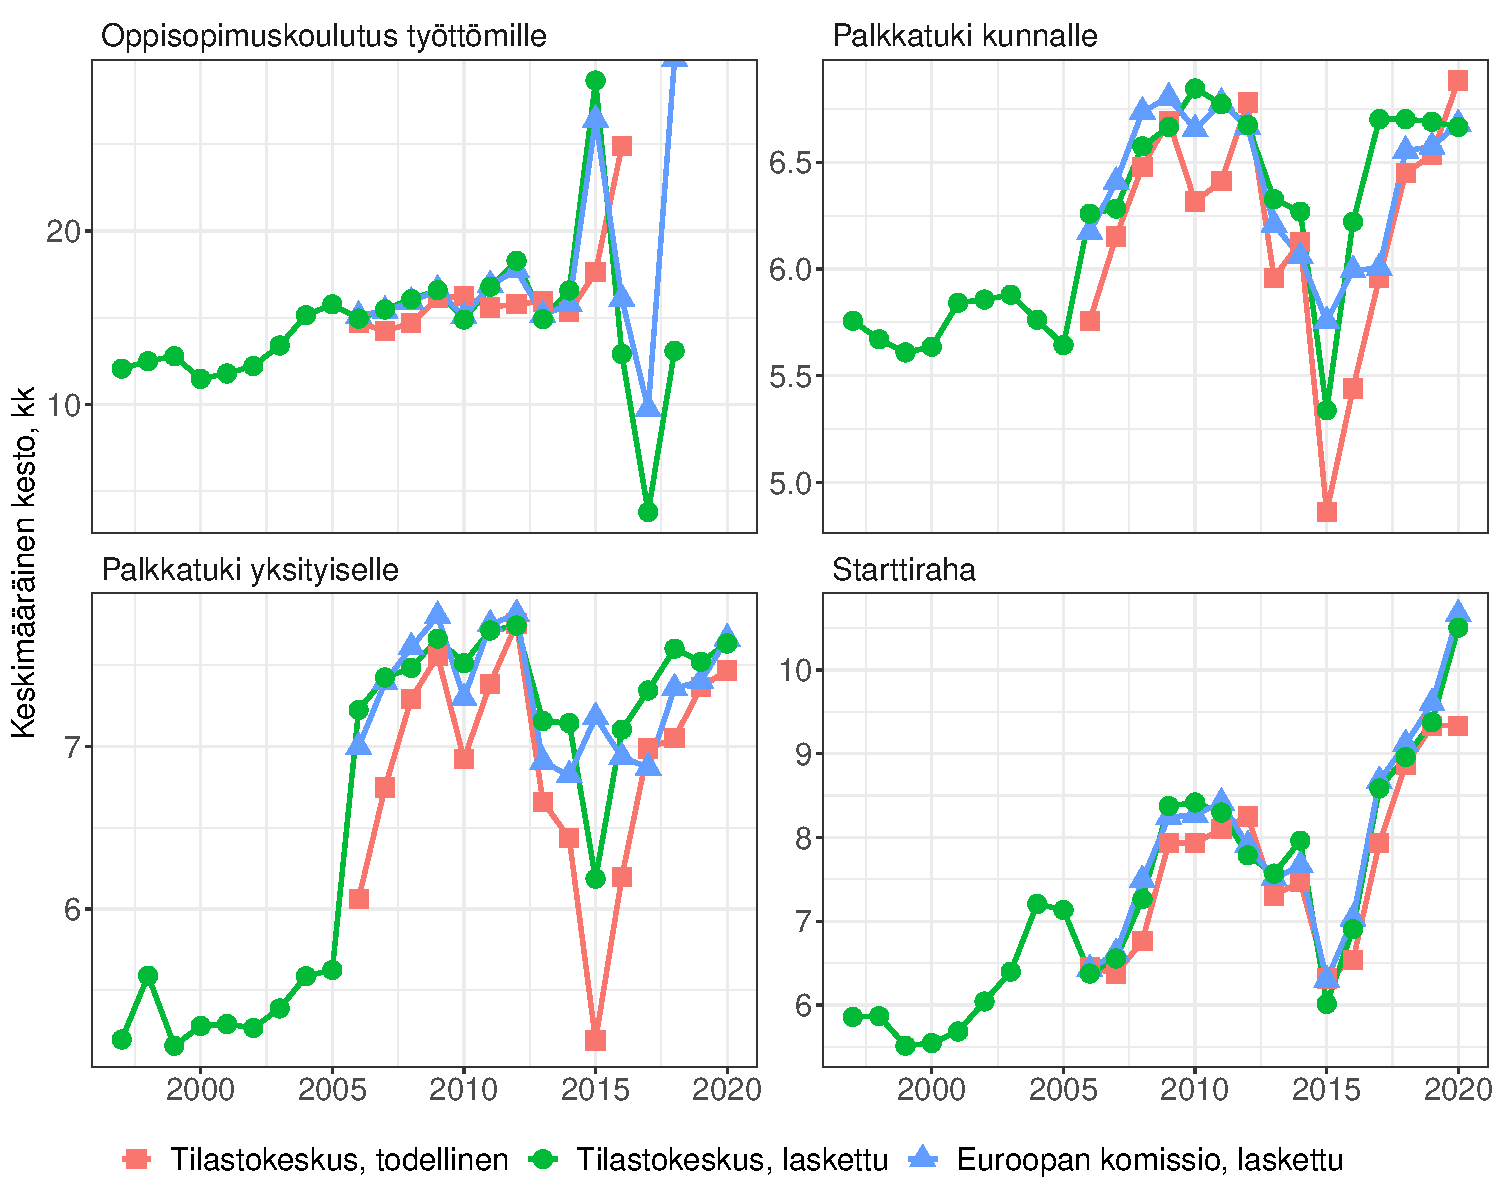
\includegraphics[scale = 0.6]{../plots/durations/tyollistaminen.pdf}
\caption{Palveluiden keskimääräinen kesto, työllistäminen. \captionselite{\protect \seliteduration{tyollistaminen} Euroopan komissio, laskettu, kuten Kuvio \ref{fig:sk230923t}. Kirjoittajan omat laskelmat.}}
   \label{fig:0bn233t}
\end{figure}

\begin{figure}
\centering
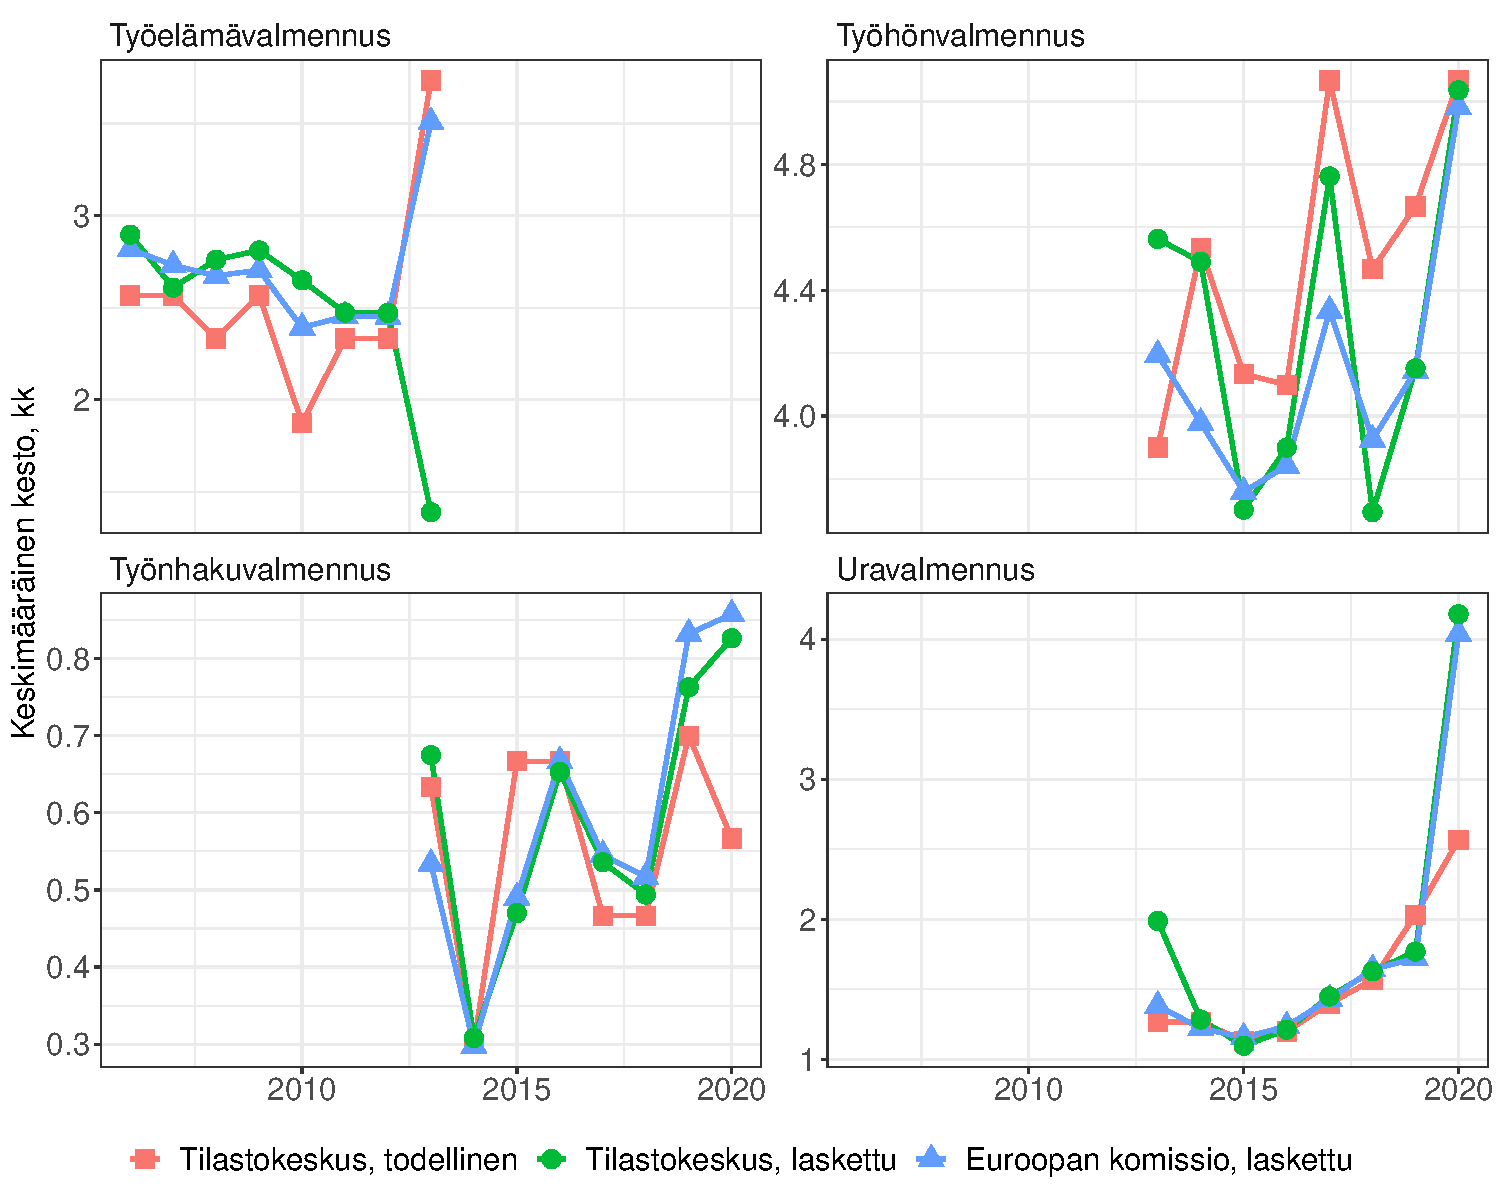
\includegraphics[scale = 0.6]{../plots/durations/valmennus.pdf}
\caption{Palveluiden keskimäärinen kesto, valmennukset. \captionselite{\protect \seliteduration{valmennus} Euroopan komissio, laskettu, kuten Kuvio \ref{fig:sk230923t}. Kirjoittajan omat laskelmat.}}
   \label{fig:9sedt23}
\end{figure}

\begin{figure}
\centering
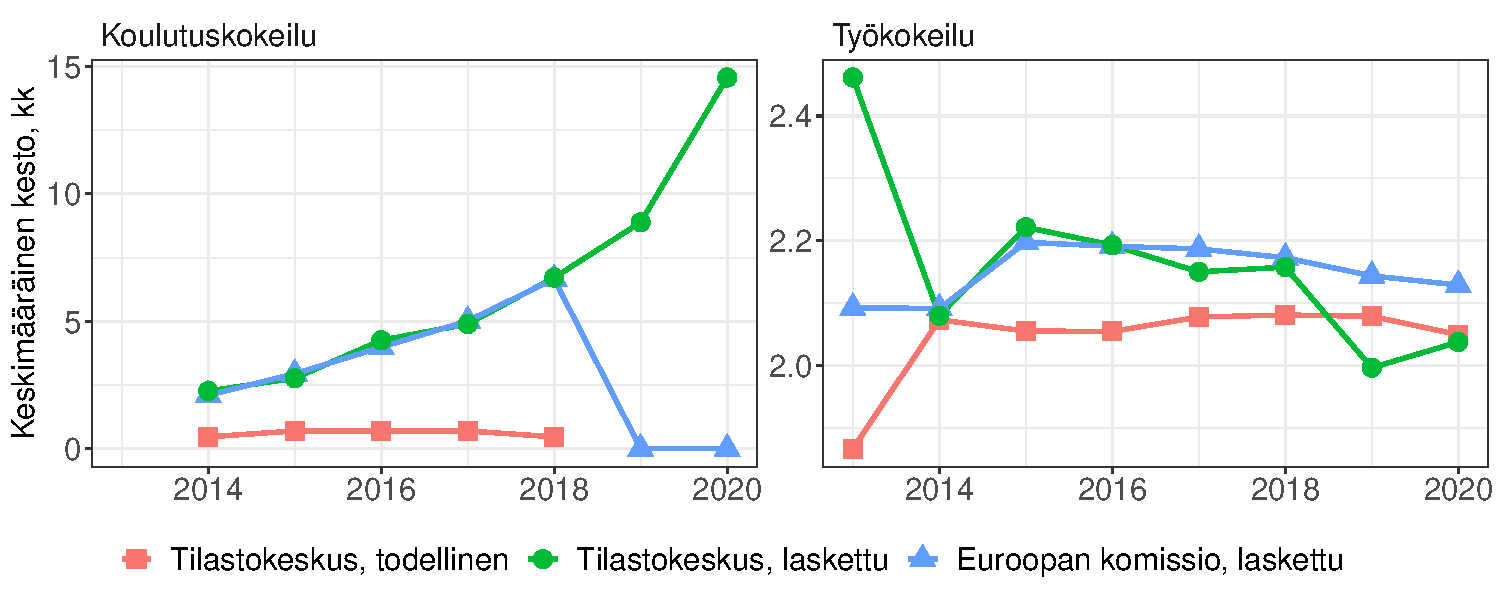
\includegraphics[scale = 0.6]{../plots/durations/kokeilu.pdf}
\caption{Palveluiden keskimääräinen kesto, kokeilut. \captionselite{\protect \seliteduration{kokeilu} Euroopan komissio, laskettu, kuten Kuvio \ref{fig:sk230923t}. Kirjoittajan omat laskelmat.}}
   \label{fig:d923t23}
\end{figure}

\begin{figure}
\centering
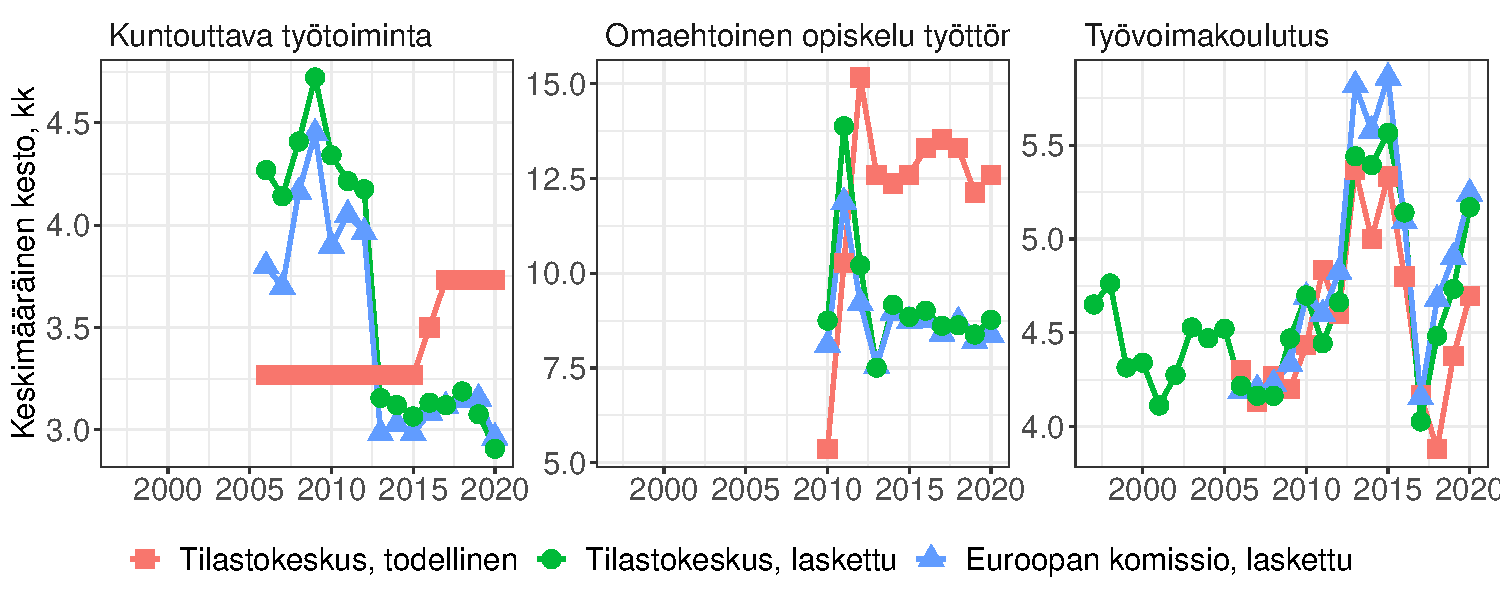
\includegraphics[scale = 0.6]{../plots/durations/muu.pdf}
\caption{Palveluiden keskimääräinen kesto, muut palvelut. \captionselite{\protect \seliteduration{muu} Euroopan komissio, laskettu, kuten Kuvio \ref{fig:sk230923t}. Kirjoittajan omat laskelmat.}}
   \label{fig:kdswdfwe}
\end{figure}



\subsection{Osallistumiskustannukset}

Kuvio \ref{fig:sk230wd} esittää osallistumiskustannukset siten että palveluiden kestot ovat arvioitu Euroopan komission aineistosta varanto- ja virtasuureiden avulla. Kuviot \ref{fig:f0982h3t}, \ref{fig:9f82gf23}, \ref{fig:dg03223} and \ref{fig:f9028yt32} tarkastelevat tulosten herkkyyttä palvelujen kestojen eri määrittely- ja laskutavoille. 

\begin{figure}[b]
\centering
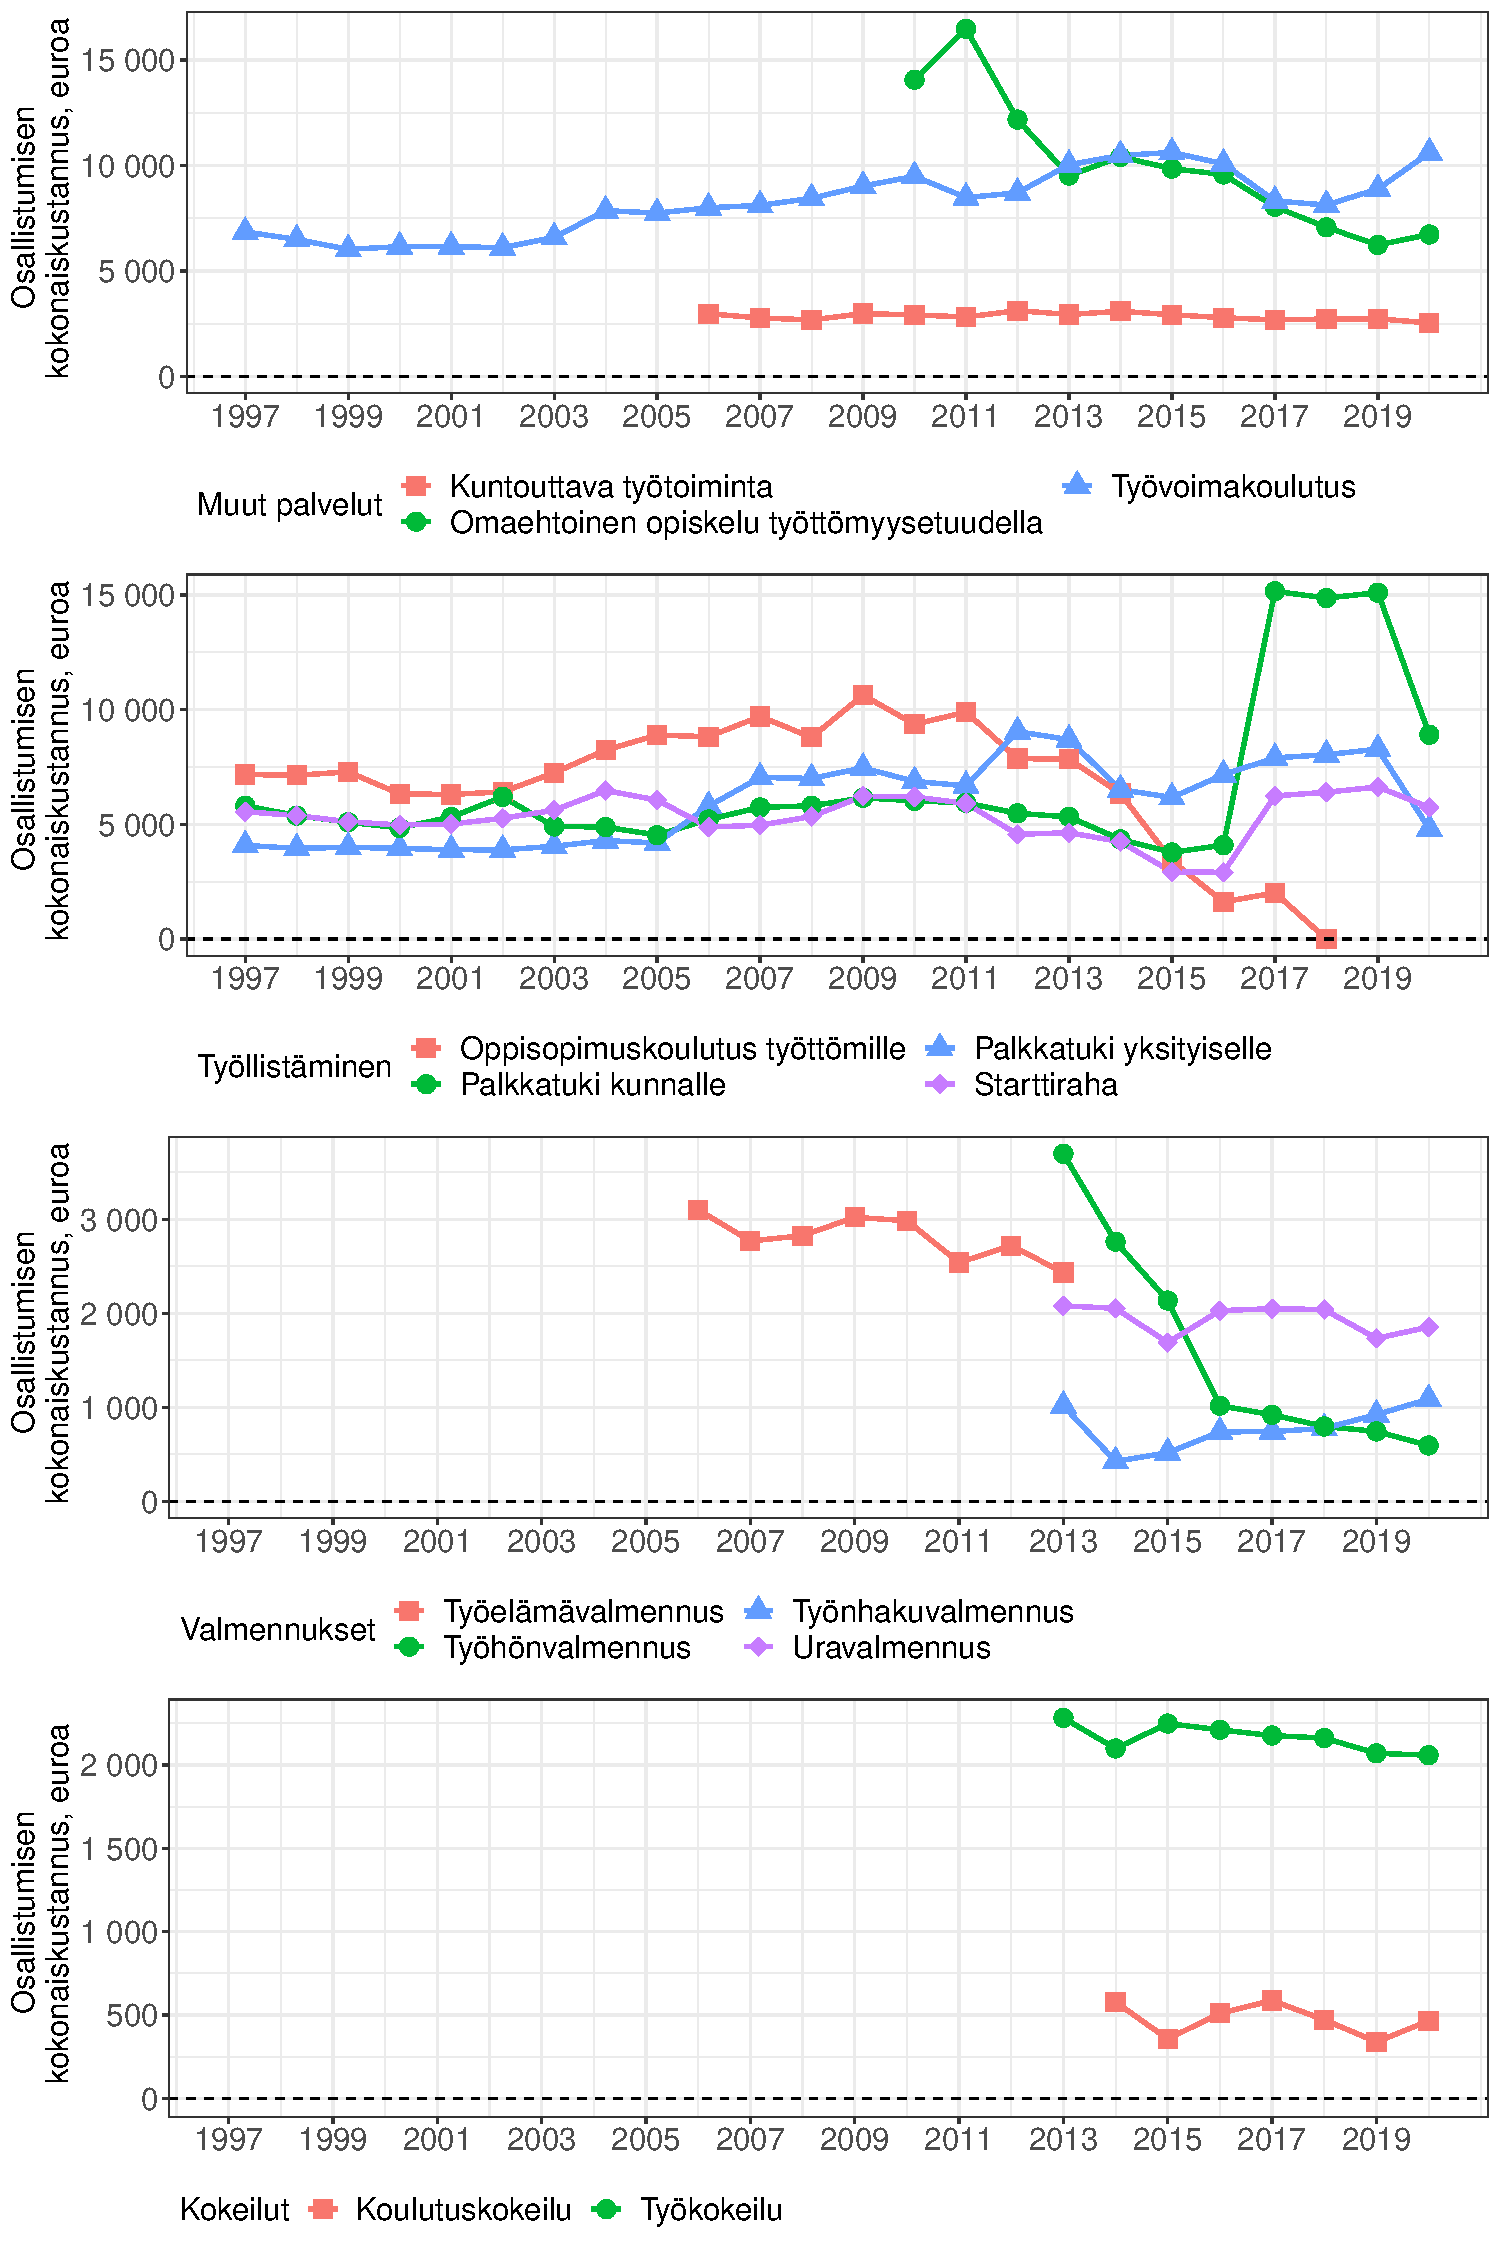
\includegraphics[scale = 0.6]{../plots/costs/participation_costs.pdf}
\caption{Osallistumiskustannukset. \captionselite{Datalähde: kuten Kuvio \ref{fig:sk230923t}. Kirjoittajan omat laskelmat.}}
   \label{fig:sk230wd}
\end{figure}


\begin{figure}
\centering
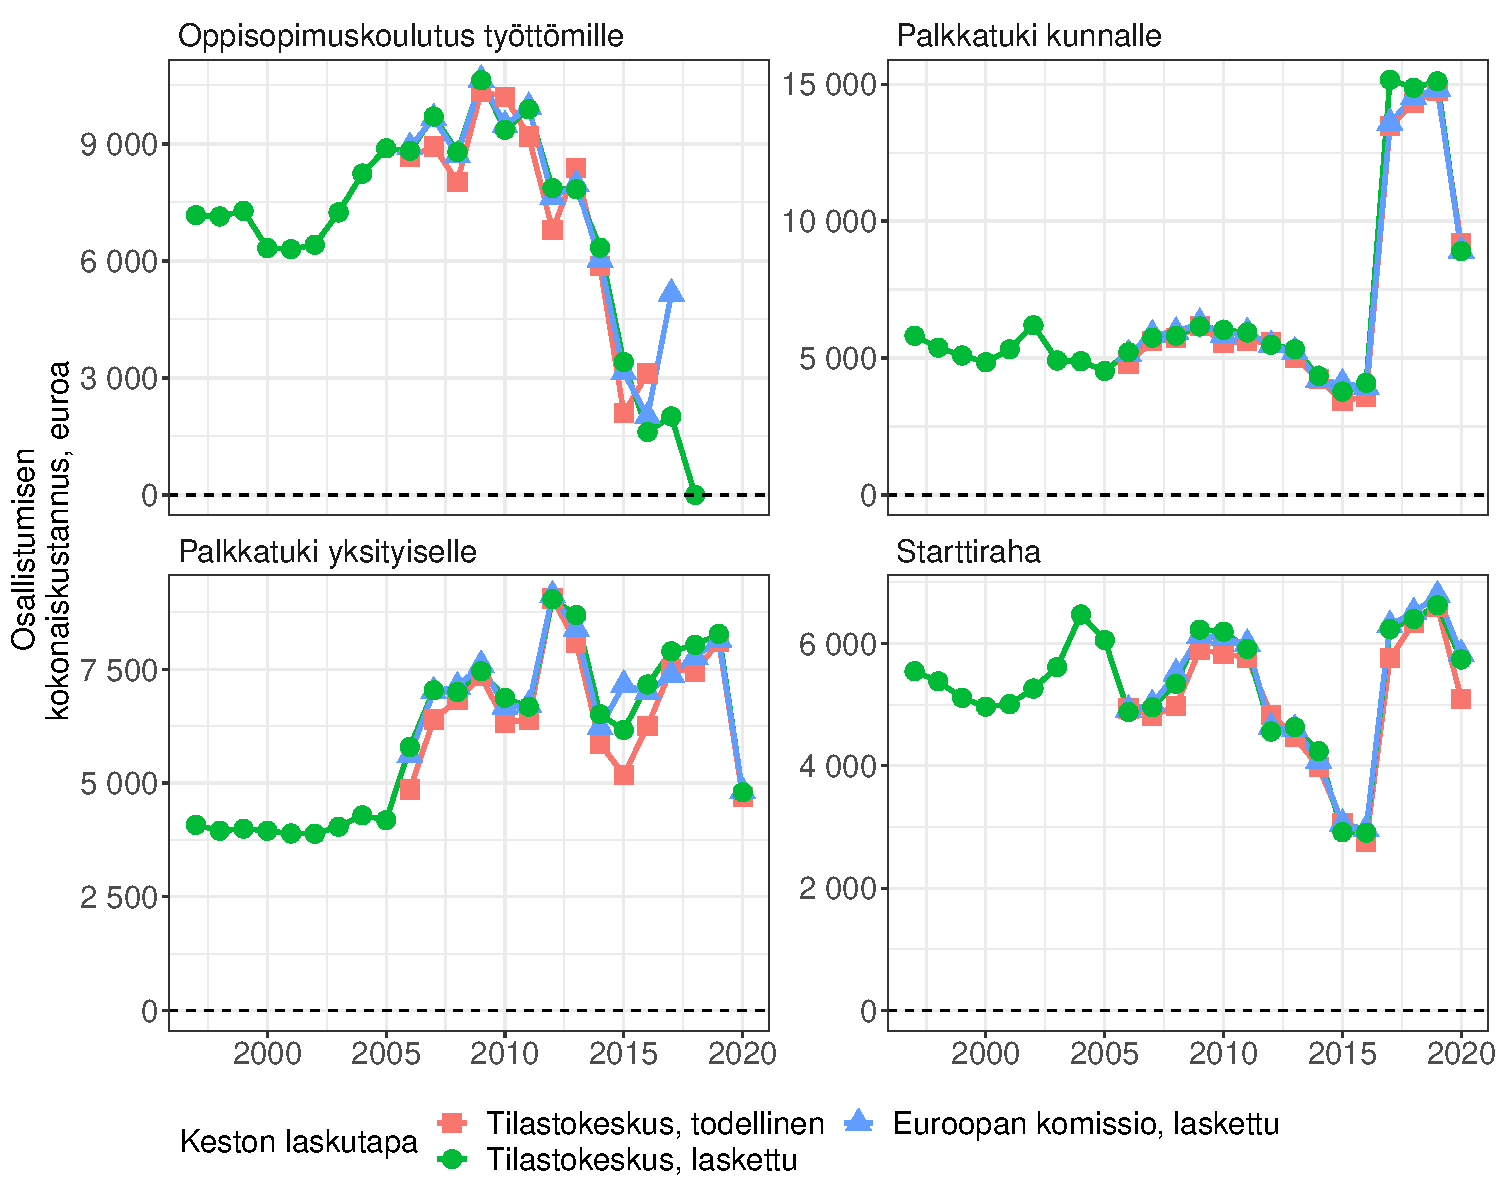
\includegraphics[scale = 0.6]{../plots/costs/tyollistaminen_robustness.pdf}
\caption{Osallistumiskustannukset, työllistäminen. \captionselite{Datalähde: palvelujen kestot kuten Kuvio \ref{fig:0bn233t}, kustannukset kuten Kuvio \ref{fig:dl2092g}}}
   \label{fig:f0982h3t}
\end{figure}

\begin{figure}
\centering
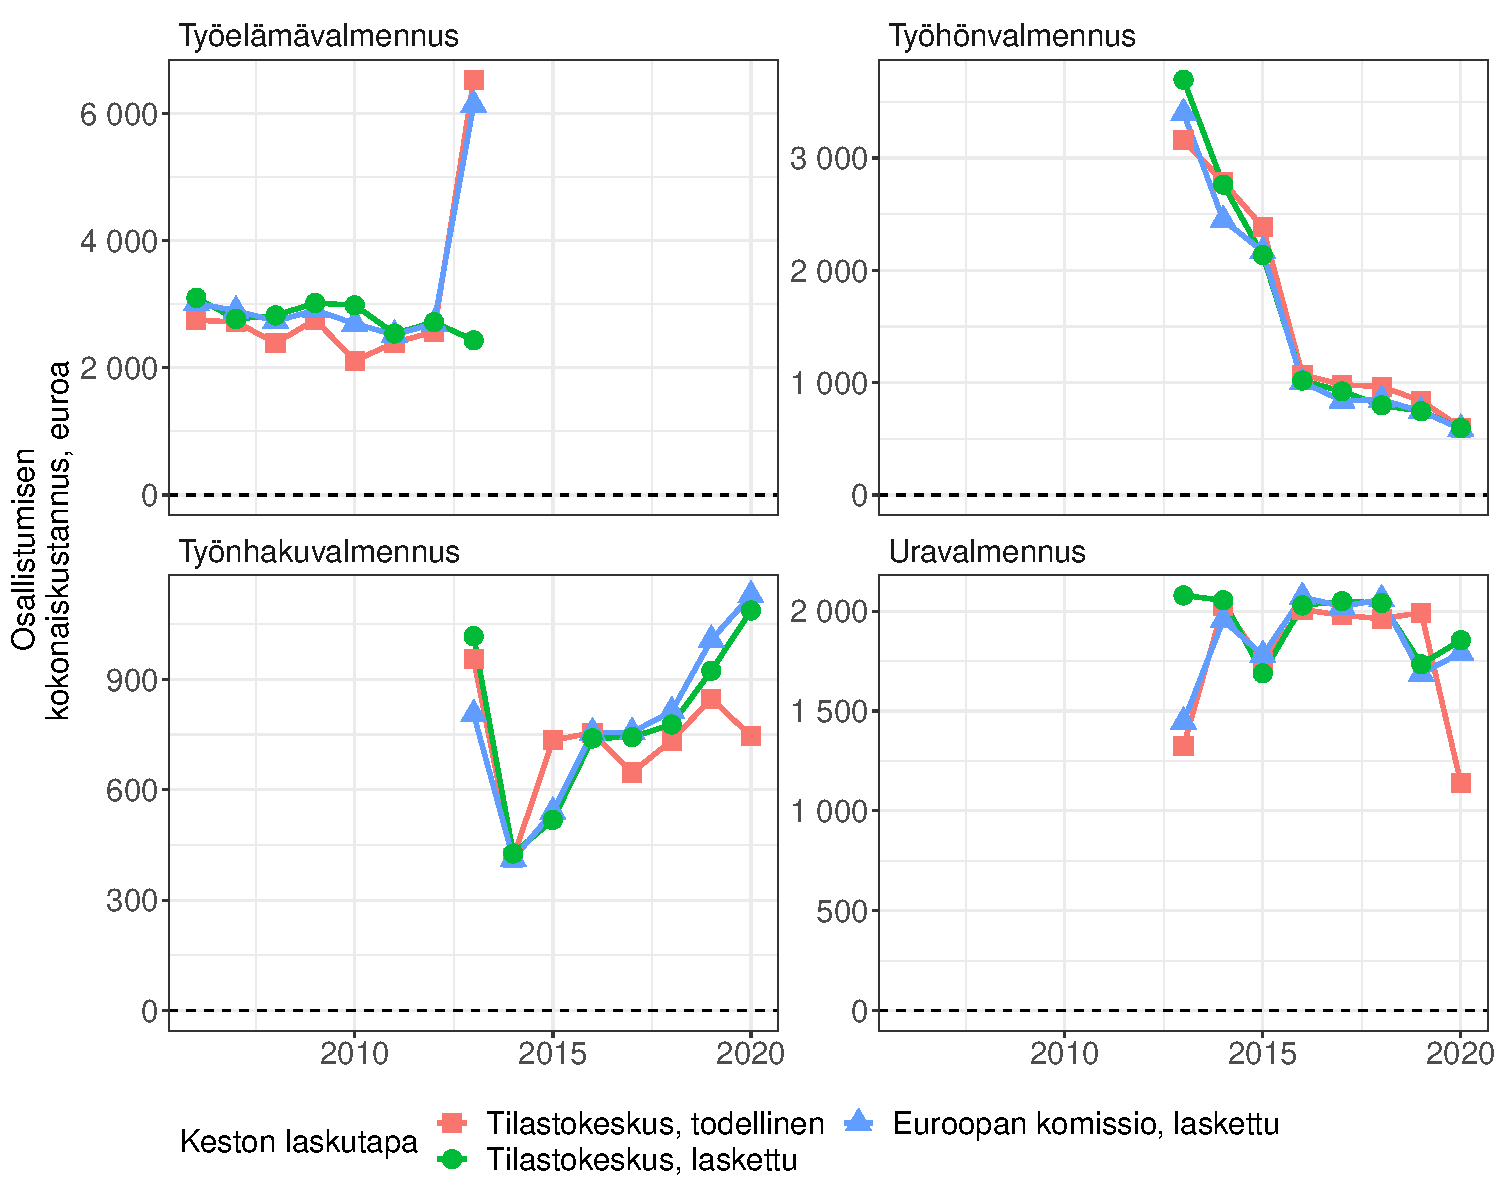
\includegraphics[scale = 0.6]{../plots/costs/valmennus_robustness.pdf}
\caption{Osallistumiskustannukset, valmennukset. \captionselite{Datalähde: palvelujen kestot kuten Kuvio \ref{fig:9sedt23}, kustannukset kuten Kuvio \ref{fig:dl2092g}}}
   \label{fig:9f82gf23}
\end{figure}

\begin{figure}
\centering
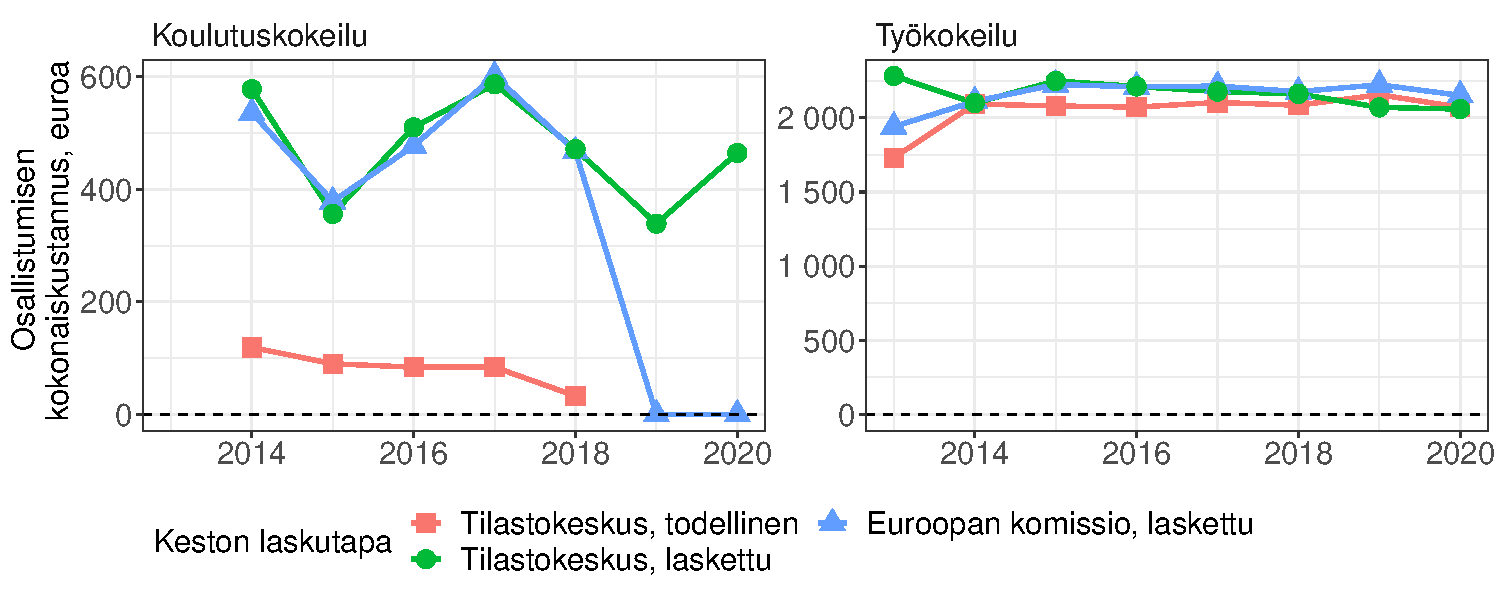
\includegraphics[scale = 0.6]{../plots/costs/kokeilu_robustness.pdf}
\caption{Osallistumiskustannukset, kokeilut. \captionselite{Datalähde: palvelujen kestot kuten Kuvio \ref{fig:d923t23}, kustannukset kuten Kuvio \ref{fig:dl2092g}}}
   \label{fig:dg03223}
\end{figure}

\begin{figure}
\centering
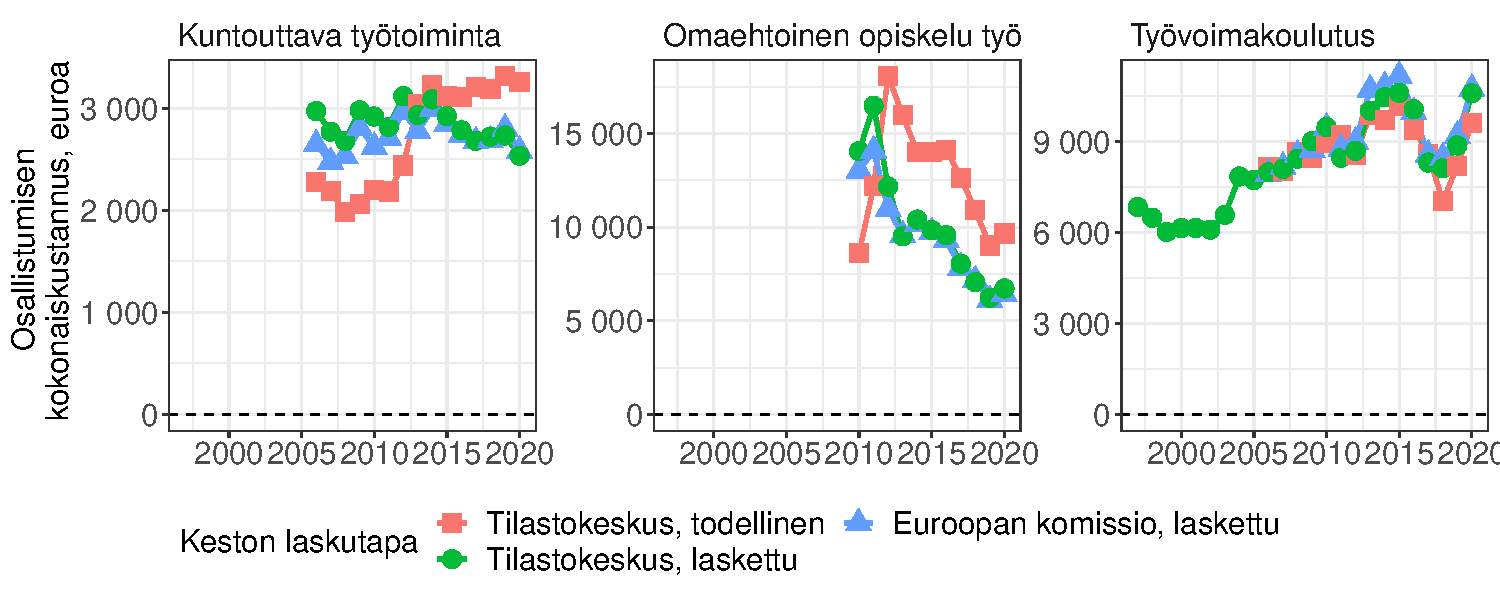
\includegraphics[scale = 0.6]{../plots/costs/muu_robustness.pdf}
\caption{Osallistumiskustannukset, muut palvelut. \captionselite{Datalähde: palvelujen kestot kuten Kuvio \ref{fig:kdswdfwe}, kustannukset kuten Kuvio \ref{fig:dl2092g}}}
   \label{fig:f9028yt32}
\end{figure}

\end{document}